\chapter{Cơ sở lý thuyết}
\label{chap:chap3}
Chương này sẽ cung cấp nền tảng cơ sở lí thuyết cho đề tài với các nội dung sau:
\begin{itemize}
    \item Công nghệ Blockchain và Ethereum
    \item Giải pháp ZK-Rollup và token ERC-20
    \item zk-SNARKs và Groth16
    \item Trình biên dịch Circom và các mức tối ưu hoá ràng buộc
    \item Phân tích mức tối ưu hoá --O2
\end{itemize}
\section{Công nghệ Blockchain và Ethereum}
\subsection{Khái niệm}
Blockchain là một công nghệ sổ cái phân tán (Distributed Ledger Technology -- DLT) cho phép ghi chép thông tin các giao dịch một cách an toàn, minh bạch và bất biến. Thay vì lưu trữ dữ liệu tập trung trên một máy chủ duy nhất, blockchain phân tán các bản sao của sổ cái trên một mạng lưới các máy tính (node). Mỗi bản ghi giao dịch sẽ được gom lại thành các ``khối'' (blocks), và các khối này được liên kết với nhau theo trình tự thời gian bằng mã hash, tạo thành một ``chuỗi'' liên tục. Khi một khối mới được thêm vào chuỗi, nó không thể bị thay đổi hoặc xóa bỏ, giúp bảo đảm tính toàn vẹn và bất biến của dữ liệu.
\subsection{Kiến trúc blockchain}
Kiến trúc của một blockchain gồm nhiều thành phần kết hợp với nhau để duy trì tính toàn vẹn và chức năng của hệ thống:

\begin{itemize}
    \item \textbf{Khối (Block)}: Blockchain hoạt động trên một mạng lưới phi tập trung, nơi mỗi nút mạng (node) duy trì một bản sao của toàn bộ sổ cái. Các nút này giao tiếp trực tiếp với nhau để xác minh và lan truyền thông tin các giao dịch và khối mới.
    \item \textbf{Mạng ngang hàng (Peer-to-Peer Network)}: Blockchain hoạt động trên một mạng lưới phi tập trung, nơi mỗi nút mạng (node) duy trì một bản sao của toàn bộ sổ cái. Các nút này giao tiếp trực tiếp với nhau để xác minh và truyền bá các giao dịch và khối mới.
    \item \textbf{Thuật toán đồng thuận (Consensus Mechanism)}:Để đảm bảo tất cả các nút mạng đều có cùng một bản sao của sổ cái và đồng ý về trạng thái của mạng, blockchain sử dụng các thuật toán đồng thuận. Các thuật toán phổ biến bao gồm Proof of Work (PoW) được sử dụng trong Bitcoin và Ethereum 1.0, hoặc Proof of Stake (PoS) được sử dụng trong Ethereum 2.0 và nhiều blockchain hiện đại khác.
    \item \textbf{Mật mã học (Cryptography)}:Mật mã học là nền tảng của blockchain, giúp đảm bảo tính bảo mật và toàn vẹn của dữ liệu. Các kỹ thuật như hàm băm mật mã (cryptographic hash functions) được sử dụng để liên kết các khối và chữ ký số (digital signatures) dùng để xác thực giao dịch và quyền sở hữu tài sản.
    \item \textbf{Sổ cái phân tán (Distributed Ledger)}:Là cơ sở dữ liệu chung được chia sẻ và đồng bộ hóa trên tất cả các nút mạng. Mọi giao dịch được ghi lại trên sổ cái này và có thể được kiểm tra bởi bất kỳ ai trong mạng.
\end{itemize}

\subsection{Cách hoạt động của blockchain}
Quá trình hoạt động cơ bản của một blockchain diễn ra như sau:
\begin{enumerate}
    \item \textbf{Khởi Tạo Giao Dịch:} Một người dùng tạo một giao dịch và ký số bằng khóa riêng của mình.

    \item \textbf{Truyền Bá Giao Dịch:} Giao dịch đã ký được lan truyền đến mạng lưới các nút mạng.

    \item \textbf{Xác Thực Giao Dịch:} Các nút mạng trong mạng lưới nhận giao dịch và xác minh tính hợp lệ của giao dịch này.

    \item \textbf{Tạo Khối:} Các giao dịch hợp lệ được tập hợp lại thành một khối mới.

    \item \textbf{Đồng Thuận:} Khi một nút tìm thấy một khối hợp lệ, nó sẽ lan truyền thông tin khối đó đến các nút khác trong mạng. Các nút khác xác minh khối này và nếu hợp lệ, các nút này sẽ thêm nó vào bản sao sổ cái của mình.

    \item \textbf{Liên Kết Chuỗi:} Khối mới được thêm vào chuỗi các khối hiện có, tạo thành một bản ghi bất biến của tất cả các giao dịch.
\end{enumerate}
\subsection{Các Tính Chất của Blockchain}

Blockchain sở hữu một số tính chất cốt lõi mang lại giá trị riêng của công nghệ này:

\begin{itemize}
    \item \textbf{Phi Tập Trung (Decentralization):} Không có một thực thể trung gian hay cơ quan quản lý duy nhất nào kiểm soát mạng lưới. Quyền lực và dữ liệu được phân tán trên toàn bộ các nút mạng.
    
    \item \textbf{Bất Biến (Immutability):} Một khi giao dịch đã được ghi vào một khối và khối đó đã được thêm vào chuỗi, nó không thể bị thay đổi hoặc xóa bỏ. Điều này đảm bảo tính toàn vẹn lịch sử của dữ liệu.
    
    \item \textbf{Minh Bạch (Transparency):} Mọi giao dịch trên blockchain đều công khai và có thể được kiểm tra bởi bất kỳ ai tham gia mạng lưới (mặc dù danh tính người dùng có thể được ẩn danh thông qua địa chỉ ví).
    
    \item \textbf{Bảo Mật (Security):} Nhờ việc sử dụng mật mã học mạnh mẽ và cơ chế đồng thuận, blockchain có khả năng chống lại các cuộc tấn công như tấn công 51\% (trong PoW) và đảm bảo tính an toàn của dữ liệu.
    
    \item \textbf{Không Cần Tin Cậy (Trustlessness):} Các bên tham gia không cần phải tin tưởng lẫn nhau hay một bên thứ ba. Thay vào đó, họ tin tưởng vào các quy tắc được mã hóa trong giao thức blockchain và thuật toán đồng thuận.
\end{itemize}

\subsection{Ethereum và Hợp Đồng Thông Minh (Smart Contracts)}

Ethereum là một nền tảng blockchain thế hệ thứ hai, được giới thiệu với một tính năng đột phá: khả năng triển khai hợp đồng thông minh (smart contracts). Trong khi Bitcoin chủ yếu hoạt động như một hệ thống tiền tệ kỹ thuật số, Ethereum mở rộng chức năng của blockchain để trở thành một nền tảng chuỗi khối toàn diện hơn.

Sự khác biệt cốt lõi của Ethereum so với các blockchain đời đầu như Bitcoin là:

\begin{itemize}
    \item \textbf{Máy Ảo Ethereum (Ethereum Virtual Machine - EVM):} Ethereum tích hợp EVM, một môi trường thực thi Turing-complete, cho phép các nhà phát triển viết và triển khai các chương trình phức tạp (hợp đồng thông minh) trực tiếp trên blockchain.
    
    \item \textbf{Hợp Đồng Thông Minh:} Là các đoạn mã tự thực thi được lưu trữ trên blockchain. Chúng tự động thực hiện các thao tác được lập trình sẵn khi các điều kiện được đáp ứng, mà không cần sự can thiệp của bên thứ ba. Hợp đồng thông minh mở ra cánh cửa cho vô số ứng dụng phi tập trung (DApps) như tài chính phi tập trung (DeFi), NFT, và các tổ chức tự trị phi tập trung (DAOs).
\end{itemize}

Khả năng triển khai hợp đồng thông minh của Ethereum đã tạo ra một cuộc cách mạng trong không gian blockchain, biến nó từ một công nghệ chỉ dùng cho giao dịch tiền tệ thành một nền tảng mạnh mẽ cho các ứng dụng phi tập trung phức tạp.

% \subsection{Khả năng mở rộng của blockchain}
% Khả năng mở rộng (Scalability) là một trong những thách thức trọng yếu đối với sự phát triển và ứng dụng rộng rãi của công nghệ blockchain. Về cơ bản, khả năng mở rộng đề cập đến năng lực của một hệ thống blockchain trong việc xử lý khối lượng lớn giao dịch mà không làm suy giảm hiệu năng, bao gồm tốc độ xử lý, chi phí giao dịch và trải nghiệm người dùng. Khi số lượng người dùng và khối lượng giao dịch gia tăng, các blockchain truyền thống thường gặp phải hiện tượng tắc nghẽn mạng, chi phí giao dịch cao, và thời gian xử lý chậm.

% Thách thức về khả năng mở rộng được minh họa rõ nét thông qua khái niệm ``Blockchain Trilemma'', một vấn đề được Vitalik Buterin là nhà sáng lập của blockchain lớp 1 Ethereum nêu ra, cho rằng một blockchain khó có thể tối ưu đồng thời ba yếu tố sau:

% \begin{itemize}
%     \item \textbf{Tính bảo mật (Security):} Khả năng chống lại các cuộc tấn công và đảm bảo tính toàn vẹn dữ liệu.
%     \item \textbf{Tính phân quyền (Decentralization):} Mức độ phân tán quyền kiểm soát và loại bỏ sự phụ thuộc vào các thực thể trung gian.
%     \item \textbf{Khả năng mở rộng (Scalability):} Khả năng xử lý khối lượng lớn giao dịch một cách hiệu quả.
% \end{itemize}

% Thông thường, việc cải thiện một yếu tố sẽ kéo theo sự đánh đổi ở một hoặc cả hai yếu tố còn lại. Ví dụ, các blockchain như Bitcoin và Ethereum (trước Ethereum 2.0) ưu tiên bảo mật và phân quyền, nhưng lại gặp hạn chế về thông lượng, chỉ xử lý được khoảng 7 đến 15 giao dịch mỗi giây (TPS).

% Để giải quyết bài toán này, nhiều giải pháp về khả năng mở rộng đã được nghiên cứu và triển khai, bao gồm:
% \begin{itemize}
%     \item Giải pháp lớp 1 (On-chain Scaling): Nâng cấp trực tiếp trên blockchain cơ sở, như tăng kích thước khối, cải thiện thuật toán đồng thuận (ví dụ: Ethereum chuyển từ Proof of Work sang Proof of Stake).
%     \item Giải pháp lớp 2 (Off-chain Scaling): Di chuyển phần lớn khối lượng giao dịch ra khỏi blockchain chính, chỉ lưu trữ dữ liệu tối thiểu trên chuỗi. Các công nghệ lớp 2 tiêu biểu bao gồm Plasma, State Channels, Optimistic Rollup, và đặc biệt là Zero-Knowledge Rollup (ZK-Rollup) – một phương pháp dựa trên bằng chứng không kiến thức giúp giảm tải cho blockchain lớp 1 trong khi vẫn kế thừa tính bảo mật.
% \end{itemize}

% Ngoài ra, các chiến lược sharding cũng được nghiên cứu nhằm phân chia dữ liệu và xử lý song song, mặc dù đi kèm với những thách thức về bảo mật và đồng thuận.

% Khả năng mở rộng tiếp tục là một chủ đề nghiên cứu sôi động trong lĩnh vực blockchain, đóng vai trò then chốt trong việc hiện thực hóa các hệ sinh thái phi tập trung có quy mô lớn và ứng dụng vào các lĩnh vực như tài chính phi tập trung (DeFi), chuỗi cung ứng, và các nền tảng xã hội phi tập trung trong tương lai.

\subsection {Khả năng mở rộng của Blockchain (Blockchain Scalability)}
Cùng với sự gia tăng nhanh chóng về số lượng người dùng và ứng dụng trên blockchain, khả năng mở rộng (scalability) đã trở thành một trong những thách thức kỹ thuật then chốt đối với sự phát triển bền vững của công nghệ này. Khả năng mở rộng phản ánh năng lực của hệ thống trong việc xử lý khối lượng lớn giao dịch mà vẫn duy trì hiệu suất, chi phí hợp lý và đảm bảo trải nghiệm mượt mà cho người dùng cuối. Đây là yêu cầu bắt buộc để blockchain có thể phục vụ các ứng dụng có quy mô lớn và đáp ứng nhu cầu thực tế trong nhiều lĩnh vực khác nhau.

Tuy nhiên, việc đạt được khả năng mở rộng hiệu quả không đơn giản, do sự tồn tại của một giới hạn nền tảng được biết đến với tên gọi \textbf{Blockchain Trilemma}. Theo khái niệm này, một blockchain khó có thể tối ưu đồng thời cả ba yếu tố cốt lõi:
\begin{enumerate}
    \item \textbf{Tính bảo mật (Security):} Đảm bảo hệ thống an toàn trước các hành vi gian lận và tấn công.
    \item \textbf{Tính phân quyền (Decentralization):} Duy trì quyền kiểm soát phân tán, tránh sự phụ thuộc vào các thực thể trung gian.
    \item \textbf{Khả năng mở rộng (Scalability):} Tăng thông lượng và giảm độ trễ trong xử lý giao dịch.
\end{enumerate}

Thông thường, việc tối ưu hóa hai yếu tố đầu tiên – bảo mật và phân quyền – sẽ kéo theo sự đánh đổi về khả năng mở rộng. Thực tế, các blockchain phổ biến như Bitcoin hay Ethereum (phiên bản đầu) chỉ đạt tốc độ xử lý ở mức khiêm tốn, vào khoảng vài giao dịch mỗi giây, không đáp ứng được nhu cầu của các ứng dụng quy mô lớn.

Nguồn gốc chính của vấn đề này đến từ đặc điểm hoạt động của các mạng blockchain phân tán, nơi mọi nút trong mạng đều phải xử lý và lưu trữ toàn bộ dữ liệu giao dịch. Điều này đảm bảo tính toàn vẹn và bảo mật nhưng đồng thời làm gia tăng tải tính toán và dữ liệu theo thời gian.

Để giải quyết những giới hạn trên, nhiều chiến lược mở rộng đã được đề xuất và triển khai, bao gồm:

\begin{itemize}
    \item \textbf{Các giải pháp mở rộng trên chuỗi (Layer 1 Scaling):} Thực hiện cải tiến trực tiếp trong thiết kế blockchain cơ sở, như mở rộng kích thước khối, hoặc chuyển đổi thuật toán đồng thuận (ví dụ Ethereum chuyển sang sử dụng Proof of Stake).
    \item \textbf{Các giải pháp mở rộng ngoài chuỗi (Layer 2 Scaling):} Các giải pháp mở rộng ngoài chuỗi (Layer 2 Scaling): Đưa phần lớn giao dịch ra khỏi blockchain chính, chỉ sử dụng chuỗi cơ sở để lưu trữ các bằng chứng bảo mật cần thiết. Tiêu biểu trong nhóm này là các công nghệ Rollup (Optimistic Rollup, ZK-Rollup), Plasma, và State Channels.
    \item \textbf{Phân mảnh (Sharding):}  Chia nhỏ dữ liệu và nhiệm vụ xử lý thành các phần (shard) độc lập nhằm tăng khả năng xử lý song song, mặc dù đi kèm những thách thức riêng về tính nhất quán và bảo mật.
\end{itemize}

Khả năng mở rộng blockchain không chỉ là một vấn đề kỹ thuật đơn lẻ mà là một bài toán cân bằng giữa các mục tiêu cốt lõi trong thiết kế hệ thống. Các nghiên cứu và ứng dụng trong lĩnh vực này tiếp tục đóng vai trò trung tâm trong lộ trình phát triển các nền tảng blockchain thế hệ tiếp theo.
 

\section{Giải Pháp ZK-Rollup và Token ERC-20}

\subsection{Khái Niệm ZK-Rollup}
ZK-Rollup (Zero-Knowledge Rollup) là một giải pháp mở rộng quy mô lớp 2 (Layer 2) cho các blockchain nền tảng (Layer 1) như Ethereum. Mục tiêu chính của ZK-Rollup là tăng thông lượng và giảm chi phí giao dịch bằng cách thực hiện phần lớn các tính toán và lưu trữ dữ liệu ngoài chuỗi (off-chain), sau đó tổng hợp hàng nghìn giao dịch thành một bằng chứng mật mã duy nhất (Zero-Knowledge Proof -- ZKP) và gửi bằng chứng này lên chuỗi Layer 1 để xác minh. Điều này giúp giảm đáng kể lượng dữ liệu mà chuỗi Layer 1 phải xử lý, đồng thời vẫn đảm bảo tính bảo mật và toàn vẹn của các giao dịch off-chain.

\begin{figure}[H]
    \centering
    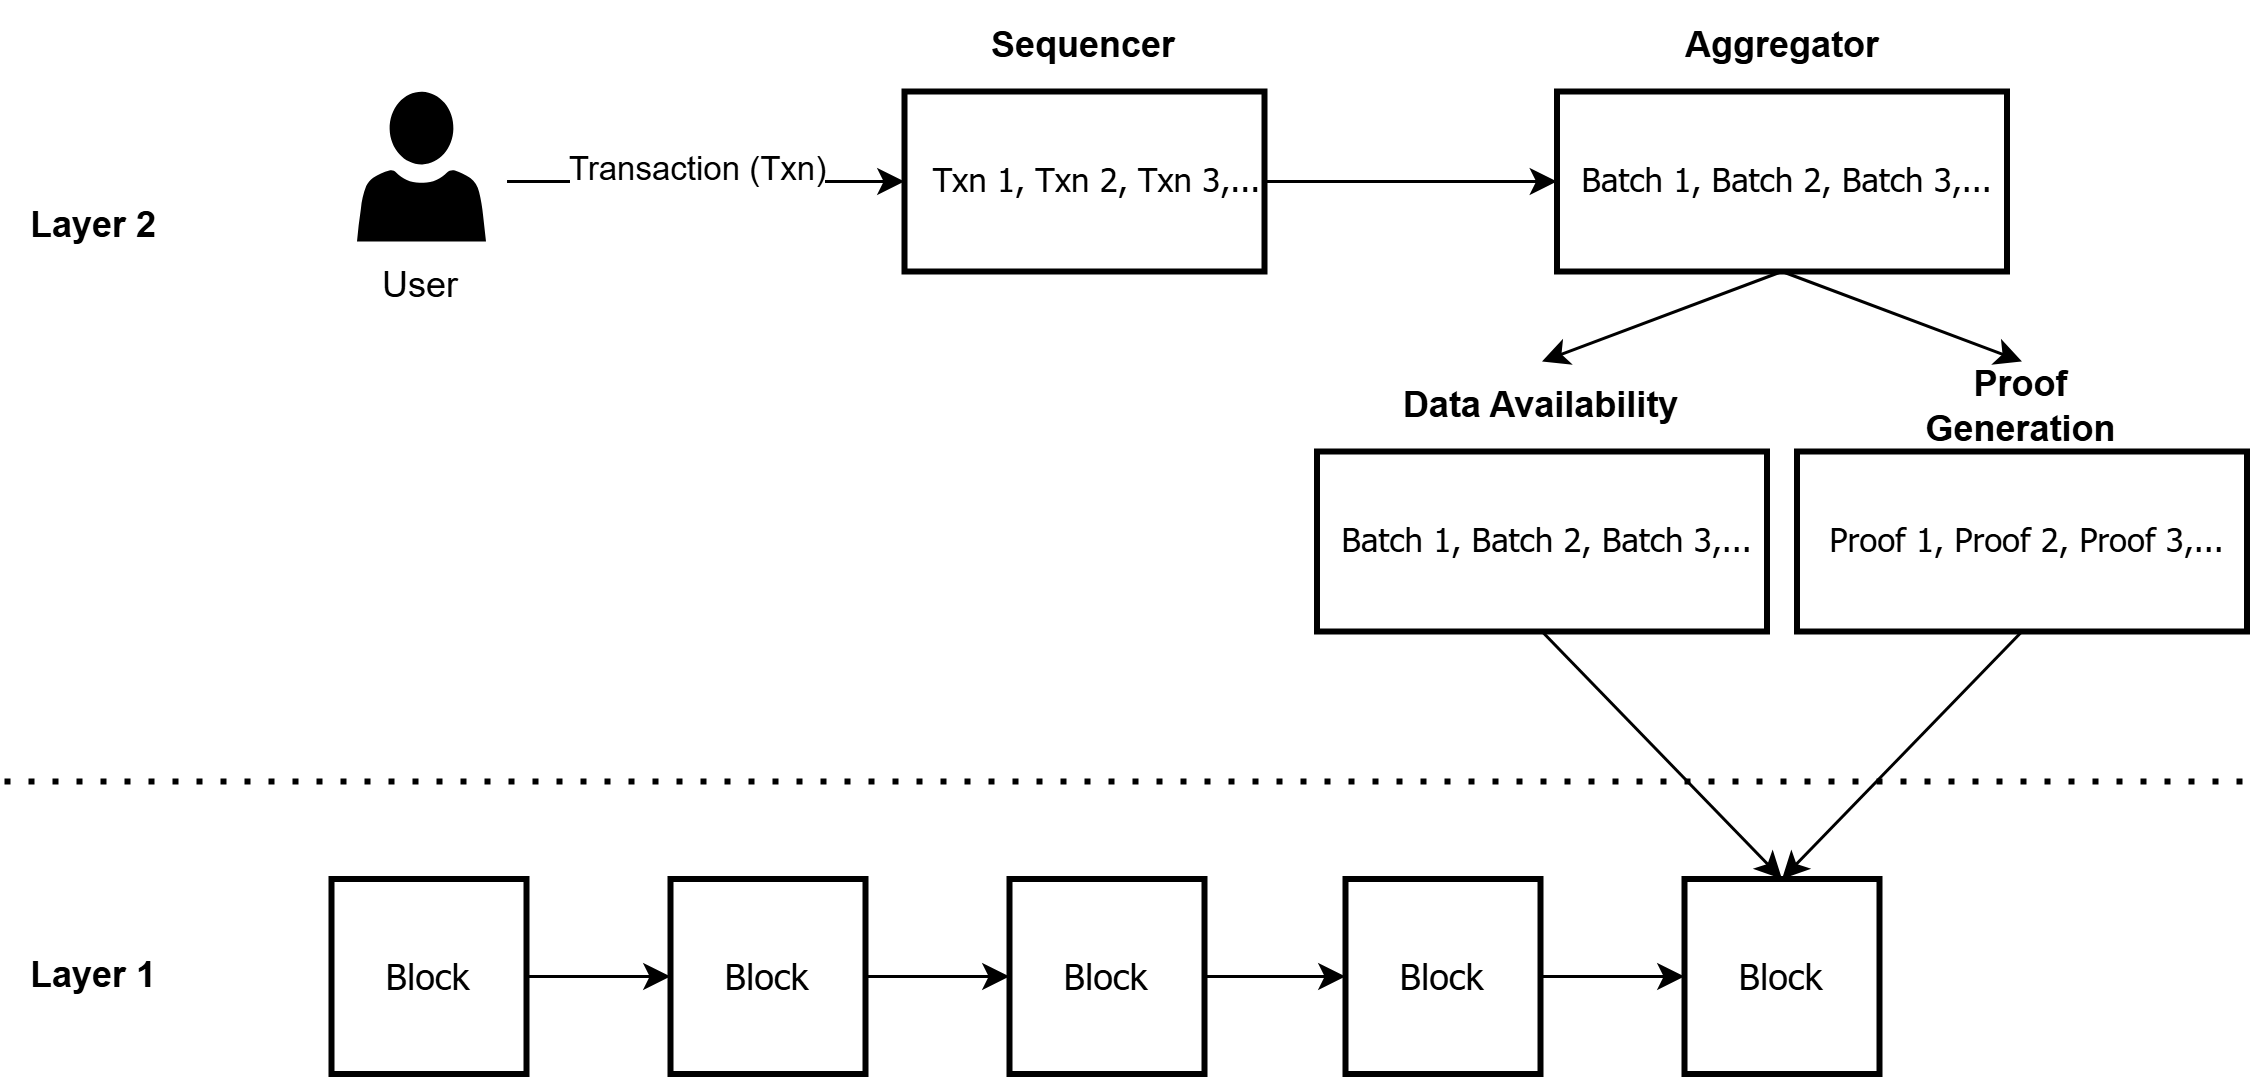
\includegraphics[width = \textwidth]{imgs/ZKRollup.png}
    \caption{Lược đồ mô tả cách ZK-Rollup hoạt động}
    \label{fig:chapter3-ZKRollup}
\end{figure}

\subsection{Cách Hoạt Động của ZK-Rollup}
Quá trình hoạt động của một hệ thống ZK-Rollup thường diễn ra như hình \ref{fig:chapter3-ZKRollup}, theo các bước sau:

\begin{enumerate}
    \item \textbf{Gửi tiền vào Rollup:} Người dùng gửi tài sản (ví dụ: token ERC-20) từ blockchain Layer 1 vào một hợp đồng thông minh trên Layer 1 được quản lý bởi ZK-Rollup. Tài sản này sau đó được ghi nhận trên ZK-Rollup ngoài chuỗi (off-chain).

    \item \textbf{Thực hiện giao dịch Off-chain:} Hàng trăm hoặc hàng nghìn giao dịch (ví dụ: chuyển token) sẽ được thực hiện ngoài chuỗi trên mạng lưới của ZK-Rollup. Các giao dịch này được tổng hợp và xử lý bởi một thực thể gọi là ``bộ tổng hợp'' (sequencer hoặc aggregator).

    \item \textbf{Tạo bằng chứng không kiến thức (ZKP):} Sau khi xử lý một lô (batch) giao dịch, bộ tổng hợp tạo ra một bằng chứng ZKP chứng minh rằng tất cả các giao dịch trong lô đó đều hợp lệ và đã được thực hiện đúng cách. Bằng chứng này rất nhỏ gọn và không tiết lộ bất kỳ thông tin chi tiết nào về các giao dịch riêng lẻ, chỉ xác nhận tính đúng đắn của chúng.

    \item \textbf{Gửi bằng chứng lên Layer 1:} Bằng chứng ZKP cùng với một bản tóm tắt nhỏ gọn về trạng thái mới của Rollup (ví dụ: gốc Merkle mới của cây trạng thái) được gửi lên hợp đồng thông minh của ZK-Rollup trên chuỗi Layer 1.

    \item \textbf{Xác minh trên Layer 1:} Hợp đồng thông minh trên Layer 1 xác minh bằng chứng ZKP. Quá trình xác minh này rất nhanh chóng và hiệu quả, bất kể số lượng giao dịch trong lô là bao nhiêu. Nếu bằng chứng hợp lệ, trạng thái mới của Rollup được cập nhật trên Layer 1, và các giao dịch trong lô được coi là đã hoàn tất.
\end{enumerate}

\subsection{Lợi Ích của ZK-Rollup}
ZK-Rollup mang lại nhiều lợi ích quan trọng cho các blockchain Layer 1:

\begin{itemize}
    \item \textbf{Khả năng mở rộng:} Bằng cách xử lý hàng nghìn giao dịch off-chain và chỉ gửi một bằng chứng duy nhất lên Layer 1, ZK-Rollup tăng đáng kể thông lượng giao dịch của blockchain nền tảng.

    \item \textbf{Giảm chi phí giao dịch:} Do ít dữ liệu được ghi lên Layer 1 hơn, phí gas cho mỗi giao dịch riêng lẻ trên ZK-Rollup được giảm thiểu đáng kể.

    \item \textbf{Bảo mật cao:} ZK-Rollup kế thừa tính bảo mật của Layer 1. Bằng chứng không kiến thức đảm bảo rằng tất cả các giao dịch off-chain đều hợp lệ về mặt mật mã, và không thể có giao dịch gian lận nào được chấp nhận trên Layer 1. Điều này khác với Optimistic Rollup, vốn dựa vào một khoảng thời gian tranh chấp.

    \item \textbf{Tính hoàn thiện tức thì (Instant Finality):} Một khi bằng chứng ZKP được xác minh trên Layer 1, các giao dịch trong lô được coi là hoàn tất ngay lập tức, không cần chờ đợi thời gian tranh chấp như các giải pháp Rollup khác.
\end{itemize}

\subsection{Token ERC-20}
ERC-20 (Ethereum Request for Comment 20) \cite{erc20} là một tiêu chuẩn kỹ thuật được sử dụng để tạo và phát hành các token có thể thay thế (fungible tokens) trên blockchain Ethereum. Tiêu chuẩn này định nghĩa một tập hợp các quy tắc chung mà tất cả các token ERC-20 phải tuân thủ, bao gồm các chức năng như chuyển token, phê duyệt chi tiêu, kiểm tra số dư, và tổng cung. Nhờ có tiêu chuẩn này, các token ERC-20 có thể tương tác dễ dàng với các ứng dụng phi tập trung (DApps), ví điện tử, sàn giao dịch và các hợp đồng thông minh khác trong hệ sinh thái Ethereum.

\subsection{Vai trò của Token ERC-20 trong ZK-Rollup}
Các giao dịch liên quan đến token ERC-20 là một trong những trường hợp sử dụng phổ biến và quan trọng nhất của ZK-Rollup. Với một số lí do sau:

\begin{itemize}
    \item \textbf{Khối lượng giao dịch lớn:} Các token ERC-20 được sử dụng rộng rãi, nên sẽ có một lượng lớn giao dịch chuyển khoản, hoán đổi, và tương tác với các hợp đồng DeFi. Việc xử lý tất cả các giao dịch này trực tiếp trên Layer 1 (Ethereum) sẽ gây ra tắc nghẽn mạng và chi phí giao dịch cao.

    \item \textbf{Tính đồng nhất:} Do các token ERC-20 tuân thủ một tiêu chuẩn chung, việc tổng hợp và xử lý chúng trong một lô giao dịch trên ZK-Rollup trở nên hiệu quả hơn. Các mạch ZKP có thể được thiết kế để xác minh tính hợp lệ của các giao dịch ERC-20 một cách đồng nhất.

    \item \textbf{Nhu cầu tối ưu hóa:} Với sự phát triển của các ứng dụng DeFi và Web3, nhu cầu về khả năng mở rộng cho các giao dịch token là rất lớn. ZK-Rollup cung cấp một giải pháp hiệu quả để đáp ứng nhu cầu này, và việc tối ưu hóa các mạch ZKP cho giao dịch ERC-20 trực tiếp góp phần vào hiệu suất tổng thể của hệ thống.
\end{itemize}

Giải pháp ZK-Rollup đóng vai trò then chốt trong việc giải quyết bài toán khả năng mở rộng của các blockchain Layer 1, đặc biệt là đối với các giao dịch token ERC-20. Bằng cách kết hợp sức mạnh của ZKP với việc xử lý off-chain, ZK-Rollup không chỉ tăng thông lượng và giảm chi phí mà còn duy trì được tính bảo mật cao. Sự phổ biến của token ERC-20 khiến việc tối ưu hóa hiệu suất xử lý các giao dịch này trên ZK-Rollup trở thành một lĩnh vực nghiên cứu và phát triển quan trọng hiện nay, trực tiếp góp phần vào sự phát triển của hệ sinh thái blockchain.

\section{zk-SNARKs và Groth16}
\subsection{zk-SNARK}
Zero-Knowledge Succinct Non-Interactive Argument of Knowledge (zk-SNARK) \cite{ballesteros2024enhancing} là một lớp các giao thức chứng minh không kiến thức cho phép một bên (người chứng minh) chứng minh cho bên kia (người xác minh) rằng họ biết một giải pháp (chứng cứ) cho một bài toán tính toán cụ thể mà không tiết lộ bất kỳ thông tin nào về giải pháp ngoài sự tồn tại của nó.

Các đặc điểm chính của zk-SNARK bao gồm tính ngắn gọn, bằng chứng được tạo ra rất nhỏ và có thể được xác minh một cách nhanh chóng, và tính không tương tác, có nghĩa là quá trình chứng minh và xác minh chỉ yêu cầu một thông điệp duy nhất từ người chứng minh đến người xác minh. Những đặc điểm này làm cho zk-SNARK đặc biệt phù hợp cho các ứng dụng blockchain, nơi mà hiệu suất xác minh và dung lượng lưu trữ là những yếu tố quan trọng.

Dưới đây là cấu trúc cơ bản của một hệ thống zk-SNARK trong thực tế, giải thích cho hình minh hoạ \ref{fig:chapter2-SNARKs_realworld}:
\begin{enumerate}
    \item \textbf{Lớp Mạch ZK:} Các lập trình viên sẽ viết mạch biểu diễn các logic sử dụng các ngôn ngữ thân thiện với SNARK như các ngôn ngữ DSL (Domain-Specific Language) như Circom, hoặc ngôn ngữ eDSL (Embedded Domain-Specific Language) như Halo2. Các mạch sẽ có hai nhiệm vụ: Đầu tiên dùng để tính toán các giá trị và tạo ra chứng cứ (witness), tiếp theo các mạch sẽ được dùng để kiểm tra tính chính xác của các chứng cứ.
    \item \textbf{Lớp Front-end:} Lớp này thường được thể hiện dưới dạng một trình biên dịch, với đầu vào là các mạch đã được viết, và đầu ra sẽ là các ràng buộc dưới dạng biểu diễn số học, ví dụ như R1CS. Front-end cũng cung cấp chức năng tạo chứng cứ (witness), sẽ nhận vào các giá trị công khai và riêng tư, kết hợp với mạch được viết và tạo ra chứng cứ (witness) tương ứng.
    \item \textbf{Lớp Back-end:} Lớp này thường được thể hiện dưới dạng một công cụ tạo bằng chứng như Snarkjs. Hỗ trợ các chức năng bao gồm: thiết lập đáng tin cậy, tạo ZKP và kiểm tra ZKP.
    \item \textbf{Lớp tích hợp (Integration Layer):} Ngoài các mạch cùng với front-end và back-end để tạo và chứng minh ZKP. Các ứng dụng thực tế thường yêu cầu thêm các phần hỗ trợ để tương tác với các thành phần SNARK ở trên. Một ví dụ với blockchain là các smart contract với chức năng xác minh nhằm xác minh các ZKP được gửi lên và thực thi logic tương ứng dựa trên kết quả xác minh.
\end{enumerate}

\subsection{Groth16}
Groth16 là một trong những giao thức zk-SNARK được sử dụng rộng rãi nhất hiện nay, được đề xuất bởi Jens Groth vào năm 2016 \cite{groth2016size}. Groth16 nổi bật nhờ một số lợi thế:
\begin{itemize}
    \item Bằng chứng cực kỳ ngắn gọn: Nó chỉ bao gồm ba phần tử trên một đường cong elliptic \cite{zhu2025extending}, bất kể kích thước của mạch.
    \item Thời gian xác minh nhanh: Quá trình xác minh chỉ yêu cầu một vài phép toán ghép cặp trên đường cong elliptic, làm cho nó phù hợp với các môi trường blockchain bị hạn chế về tài nguyên.
    \item Không tương tác: Nó chỉ yêu cầu một thông điệp từ người chứng minh đến người xác minh.
    \item Hỗ trợ cho các mạch phức tạp: Nó có thể được áp dụng cho các mạch lớn với nhiều ràng buộc, làm cho nó phù hợp với các ứng dụng như ZK-Rollup.
\end{itemize}

Tuy nhiên, Groth16 yêu cầu một giai đoạn thiết lập tin cậy cho mỗi mạch, và nếu bị xâm phạm, nó có thể ảnh hưởng đến bảo mật của hệ thống. Mặc dù vậy, các giải pháp như tính toán đa bên đã được triển khai để giảm thiểu rủi ro này trong thực tế.

Nghiên cứu này đã chọn Groth16 cho các giao dịch ERC-20 trên ZK-Rollup vì tối ưu hóa thời gian xác minh và kích thước bằng chứng là rất quan trọng để đáp ứng một số lượng lớn giao dịch cùng với yêu cầu xác minh bằng chứng liên tục. Groth16 cung cấp thời gian xác minh bằng chứng rất nhanh, bất chấp độ phức tạp của mạch hay kích thước của lô giao dịch. Thêm vào đó, nó cung cấp các bằng chứng với kích thước rất nhỏ, Groth16 là một trong những hệ thống có kích thước bằng chứng nhỏ nhất hiện có \cite{partala2020non}.

Hơn nữa, Circom cũng hỗ trợ tốt với các hệ thống chứng minh zk-SNARK như Groth16, tạo điều kiện cho việc tối ưu hóa mạch và trích xuất các tham số cần thiết để thuận tiện cho việc đánh giá.

\subsection{Luồng thực hiện tạo và xác minh bằng chứng}
Luồng tạo và xác minh bằng chứng \cite{shi2023data} \cite{ernstberger2024zk} có thể được tóm tắt như sau:
\[
\text{Circuit (R1CS)} \rightarrow \text{QAP} \rightarrow \text{Trusted Setup} \rightarrow \text{Groth16 Proving} \rightarrow \text{Verifier}
\]
%\vspace{0.5em}
\begin{enumerate}
    \item \textbf{Mạch số học (Arithmetic Circuit):} Quá trình bắt đầu bằng cách biểu diễn mạch số học của một phép toán. Mạch số học này được xây dựng bằng cách sử dụng các cổng cộng và nhân, với các dây dẫn (wires) mang giá trị thuộc một trường số nguyên tố hữu hạn \( F_p \). Mạch nhận tín hiệu đầu vào để thực hiện phép cộng và nhân theo modulo một số nguyên tố \( p \). Đầu ra của mỗi phép toán sẽ tạo ra một tín hiệu, tín hiệu này có thể là tín hiệu trung gian hoặc tín hiệu đầu ra cuối cùng của quá trình tính toán. Các ngôn ngữ lập trình mạch cấp cao như Circom thường được sử dụng để mô tả các mạch này. Một mạch sẽ được định nghĩa bởi các tín hiệu công khai, tín hiệu riêng tư, và hệ thống ràng buộc R1CS sẽ mô tả các phép toán của mạch trên các tín hiệu này.
    \item \textbf{Hệ thống ràng buộc bậc 1 (R1CS -- Rank 1 Constraint System):} Ở bước tiếp theo, ta chuyển đổi mạch số học thành hệ thống R1CS. R1CS là một đại diện trung gian phổ biến cho các mạch ZKP, được sử dụng bởi các công cụ frontend như Circom và ZoKrates\cite{eberhardt2018zokrates}. Biểu diễn R1CS bao gồm một tập hợp các ràng buộc, mỗi ràng buộc có một ràng buộc bậc nhất tương ứng với một cổng nhân trong mạch, được biểu diễn dưới dạng \( a \times b = c \). Tập hợp của tất cả các ràng buộc như vậy sẽ tạo thành một hệ thống các ràng buộc cấp độ 1.
    \item \textbf{Chương trình số học bậc 2 (QAP -- Quadratic Arithmetic Program):} Để phù hợp với các kỹ thuật mã hóa zk-SNARK, hệ thống R1CS được chuyển đổi tiếp trở thành một ``Chương trình số học bậc hai'' (QAP -- Quadratic Arithmetic Program). QAP mã hóa các ràng buộc của R1CS vào các đa thức đại số, ở đây các giá trị chứng cứ (witness) sẽ được đưa vào các hệ số của những đa thức này. Nếu một chứng cứ hợp lệ tồn tại, đa thức \( Q(x) \) (được xây dựng từ chứng cứ và các ràng buộc) sẽ chia hết cho một đa thức mục tiêu \( Z(x) \) (được định nghĩa bởi cấu trúc mạch). Do đó, người chứng minh cần phải chứng minh sự tồn tại của một đa thức \( H(x) \) sao cho \( Q(x) = H(x) \times Z(x) \), mà không tiết lộ trực tiếp chứng cứ hoặc các đa thức này. Việc chuyển đổi sang QAP là một bước quan trọng để áp dụng các giao thức chứng minh không kiến thức hiệu quả và an toàn.
    \item \textbf{Thiết Lập Tin Cậy (Trusted Setup):} Giai đoạn thiết lập tin cậy là một bước quan trọng để tạo ra các khóa mật mã cần thiết cho việc tạo và xác minh bằng chứng. Đối với Groth16, quy trình này thường bao gồm hai giai đoạn. Giai đoạn 1 (Powers of Tau -- một giao thức tính toán đa bên) tạo ra các giá trị bí mật ngẫu nhiên chung cho toàn bộ hệ thống. Giai đoạn 2 (thiết lập cụ thể cho từng mạch) sử dụng kết quả từ giai đoạn 1 và cấu trúc cụ thể của mạch (thông qua QAP) để tạo ra khóa chứng minh và khóa xác minh. Việc đảm bảo tính bí mật của các giá trị ngẫu nhiên được tạo ra trong quá trình này là rất quan trọng để duy trì bảo mật của hệ thống.
    \item \textbf{Tạo bằng chứng (Proving):} Trong quá trình tạo bằng chứng, người chứng minh sử dụng khóa chứng minh (được tạo ra trong giai đoạn thiết lập tin cậy) và chứng cứ (các giá trị bí mật thỏa mãn mạch) để tạo ra một bằng chứng \( \pi \). Các giá trị đầu vào công khai cũng được cung cấp cho người xác minh sử dụng trong quá trình xác minh. Bằng chứng \( \pi \) thường có kích thước rất nhỏ.

    \item \textbf{Xác minh bằng chứng (Verifying Proof):} Cuối cùng, người xác minh sử dụng khóa xác minh (cũng được tạo ra trong giai đoạn thiết lập tin cậy), bằng chứng \( \pi \) nhận được từ người chứng minh, và các giá trị đầu vào công khai để kiểm tra tính hợp lệ của bằng chứng chứng. Quá trình xác minh thường sử dụng một số phép toán ghép cặp trên đường cong elliptic, kết quả sẽ là chấp nhận hoặc từ chối bằng chứng.
\end{enumerate}

\section{Trình biên dịch Circom và các mức tối ưu hoá ràng buộc}
\subsection{Trình biên dịch Circom}
Circom \cite{belles2022circom} \cite{munoz2023circom} là một ngôn ngữ mô tả mạch (Circuit Description Language) và là một trình biên dịch (compiler) được thiết kế đặc biệt để xây dựng các mạch số học cho các bằng chứng không kiến thức (ZKP), đặc biệt là zk-SNARKs. Circom được phát triển để đơn giản hóa quá trình thiết kế và triển khai các mạch ZKP phức tạp, vốn thường đòi hỏi kiến thức sâu về mật mã và toán học. Nó cho phép các nhà phát triển định nghĩa các tính toán dưới dạng mạch số học một cách trực quan hơn, sau đó biên dịch chúng thành định dạng R1CS (Rank-1 Constraint System) mà các hệ thống zk-SNARK có thể sử dụng.

Các đặc điểm nổi bật của Circom:
\begin{itemize}
    \item \textbf{Kiểu lập trình tương tự các ngôn ngữ lập trình phần cứng:} Kiểu lập trình mô tả trực tiếp từng ràng buộc của Circom giúp lập trình viên kiểm soát tối đa từng constraint được sinh ra, giúp tạo các bằng chứng ZK nhỏ gọn, nhanh và tiết kiệm chi phí nhất.
    \item \textbf{Tính mô-đun:} Circom hỗ trợ khái niệm "template" (mẫu), cho phép tạo ra các mạch con có thể tái sử dụng và tham số hóa. Điều này giúp xây dựng các mạch lớn hơn từ các thành phần cơ bản, tăng cường khả năng tái sử dụng mã và giảm độ phức tạp khi triển khai mạch.
    \item \textbf{Hỗ trợ biên dịch R1CS}: Chức năng chính của trình biên dịch Circom là chuyển đổi mã Circom thành một tập hợp các ràng buộc R1CS, cùng với các tệp hỗ trợ khác (như tệp wasm hoặc c++ để tính toán chứng cứ).
    \item \textbf{Hệ sinh thái:} Circom là một phần của một hệ sinh thái lớn hơn bao gồm circomlib (thư viện các template mạch phổ biến) và snarkjs (thư viện JavaScript để tạo và xác minh bằng chứng zk-SNARK) cùng các công cụ hỗ trợ khác như circomspect, circomkit,... Giúp các nhà phát triển thuận tiện hơn trong việc xây dựng các ứng dụng ZK.
    \item \textbf{Là trình biên dịch và ngôn ngữ đã phát triển và được sử dụng rộng rãi:} Circom phát triển được qua hai phiên bản ổn định với nhiều cải tiến giúp thuận tiện hơn cho người sử dụng, đồng thời đã được ứng dụng trong nhiều dự án thực tế như ứng dụng gửi tiền ẩn danh trên Ethereum Tornado Cash \cite{khovratovich2019tornado} và ZK-Rollup Hermez Network, là tiền thân của ZK-Rollup Polygon Hermez hiện nay.
\end{itemize}

\subsection{Cơ chế tối ưu hoá ràng buộc trong Circom}
\label{Cơ chế tối ưu hoá ràng buộc trong Circom}
Trong các hệ thống zk-SNARK, số lượng ràng buộc trong mạch R1CS có ảnh hưởng trực tiếp đến hiệu suất của quá trình tạo bằng chứng (proving time) và kích thước của bằng chứng (proof size). Càng ít ràng buộc, quá trình tạo bằng chứng càng nhanh và bằng chứng càng nhỏ. Circom cung cấp các cờ tối ưu hóa khác nhau để giúp giảm số lượng ràng buộc được tạo ra trong quá trình biên dịch.

Các cờ tối ưu hóa này hoạt động bằng cách áp dụng các kỹ thuật biến đổi đại số để loại bỏ các ràng buộc dư thừa hoặc đơn giản hóa các ràng buộc hiện có. Dưới đây là các mức tối ưu hóa chính được hỗ trợ bởi trình biên dịch Circom:

\begin{enumerate}
    \item \textbf{--O0 (Không tối ưu hóa):}
    \begin{itemize}
        \item Đây là mức tối ưu hóa thấp nhất, nơi trình biên dịch không áp dụng bất kỳ kỹ thuật tối ưu hóa ràng buộc nào. Mỗi phép toán trong mạch Circom sẽ được chuyển đổi trực tiếp thành các ràng buộc R1CS tương ứng mà không có sự đơn giản hóa nào.
    \end{itemize}
    \item \textbf{--O1 (Tối ưu hóa cơ bản - Mặc định):}
    \begin{itemize}
        \item Đây là mức tối ưu hóa mặc định của trình biên dịch Circom. Nó áp dụng các tối ưu hóa cơ bản nhưng hiệu quả để giảm số lượng ràng buộc.
        \item Các tối ưu hóa chính ở mức --O1 bao gồm việc loại bỏ các ràng buộc có dạng \texttt{signal = k} (trong đó \texttt{k} là một hằng số) và \texttt{signal1 = signal2}. Trình biên dịch sẽ thay thế tất cả các lần xuất hiện của \texttt{signal} bằng \texttt{k} hoặc thay \texttt{signal1} bằng \texttt{signal2} (hoặc ngược lại, tùy thuộc vào việc một trong các tín hiệu là riêng tư để duy trì tính đúng đắn của bằng chứng).
    \end{itemize}
    \item \textbf{--O2 (Tối ưu hóa nâng cao):}
    \begin{itemize}
        \item Mức --O2 bao gồm tất cả các tối ưu hóa của --O1 và áp dụng thêm các kỹ thuật tối ưu hóa nâng cao hơn, đặc biệt là sử dụng khử Gauss dạng "lười" (Lazy Form of Gaussian Elimination).
        % \item Mục tiêu của -O2 là loại bỏ càng nhiều ràng buộc tuyến tính càng tốt, đặc biệt là những ràng buộc chứa ít nhất một tín hiệu riêng tư. Sau khi áp dụng các phép thế được phát hiện bởi thuật toán, một số ràng buộc phi tuyến tính có thể trở thành tuyến tính, và quá trình khử Gauss sẽ được thực hiện lặp đi lặp lại cho đến khi không còn ràng buộc tuyến tính nào chứa tín hiệu riêng tư có thể được loại bỏ.
        % \item Trong Groth16, chi phí của phép cộng được coi là miễn phí, nghĩa là không cần tạo thêm ràng buộc khi phép cộng xuất hiện trong biểu thức. Tối ưu hóa -O2 tận dụng triệt để đặc điểm này để đơn giản hóa mạch mà không ảnh hưởng đến tính đúng đắn của bằng chứng.
        \item Nguyên lý cốt lõi của tối ưu hóa -O2 dựa trên nhận định rằng các cổng cộng (addition gates) trong mạch số học được coi là ``miễn phí'' trong các hệ thống zk-SNARK như Groth16 \cite{albert2022distilling} \cite{diaz2023extending}. Điều này có nghĩa là việc thêm các phép cộng không làm tăng số lượng ràng buộc. Tận dụng điều này, -O2 tìm cách loại bỏ các ràng buộc tuyến tính (linear constraints) bằng cách thay thế một tín hiệu (signal) trong ràng buộc đó bằng một biểu thức tuyến tính tương đương. Quá trình này được thực hiện lặp đi lặp lại cho đến khi không còn ràng buộc tuyến tính nào chứa ít nhất một tín hiệu riêng tư có thể được đơn giản hóa thêm.
        \item Cụ thể, thuật toán khử Gauss dạng lười hoạt động theo nhiều vòng lặp (rounds). Trong mỗi vòng, nó xác định các ràng buộc tuyến tính và cố gắng loại bỏ các tín hiệu bằng cách tạo ra các phép thế (substitutions). Điều đặc biệt của tính "lười" là sau một số lượng vòng lặp, khi một số phép thế được áp dụng, một số ràng buộc phi tuyến tính ban đầu có thể trở thành tuyến tính. Khi đó, thuật toán sẽ tiếp tục các vòng lặp khử Gauss cho đến khi không còn ràng buộc tuyến tính mới nào được tìm thấy hoặc đạt đến điều kiện dừng. Hình \ref{fig:chapter3-SimplficationExample} minh hoạ một trường hợp đơn giản của quá trình tối ưu ràng buộc trong mạch, trong đó "signal C" là một tín hiệu riêng tư (private signal); trong trường hợp này, trình biên dịch có thể nội suy biểu thức để giảm số lượng ràng buộc.

    \end{itemize}
\end{enumerate}

\begin{figure}[H]
    \centering
    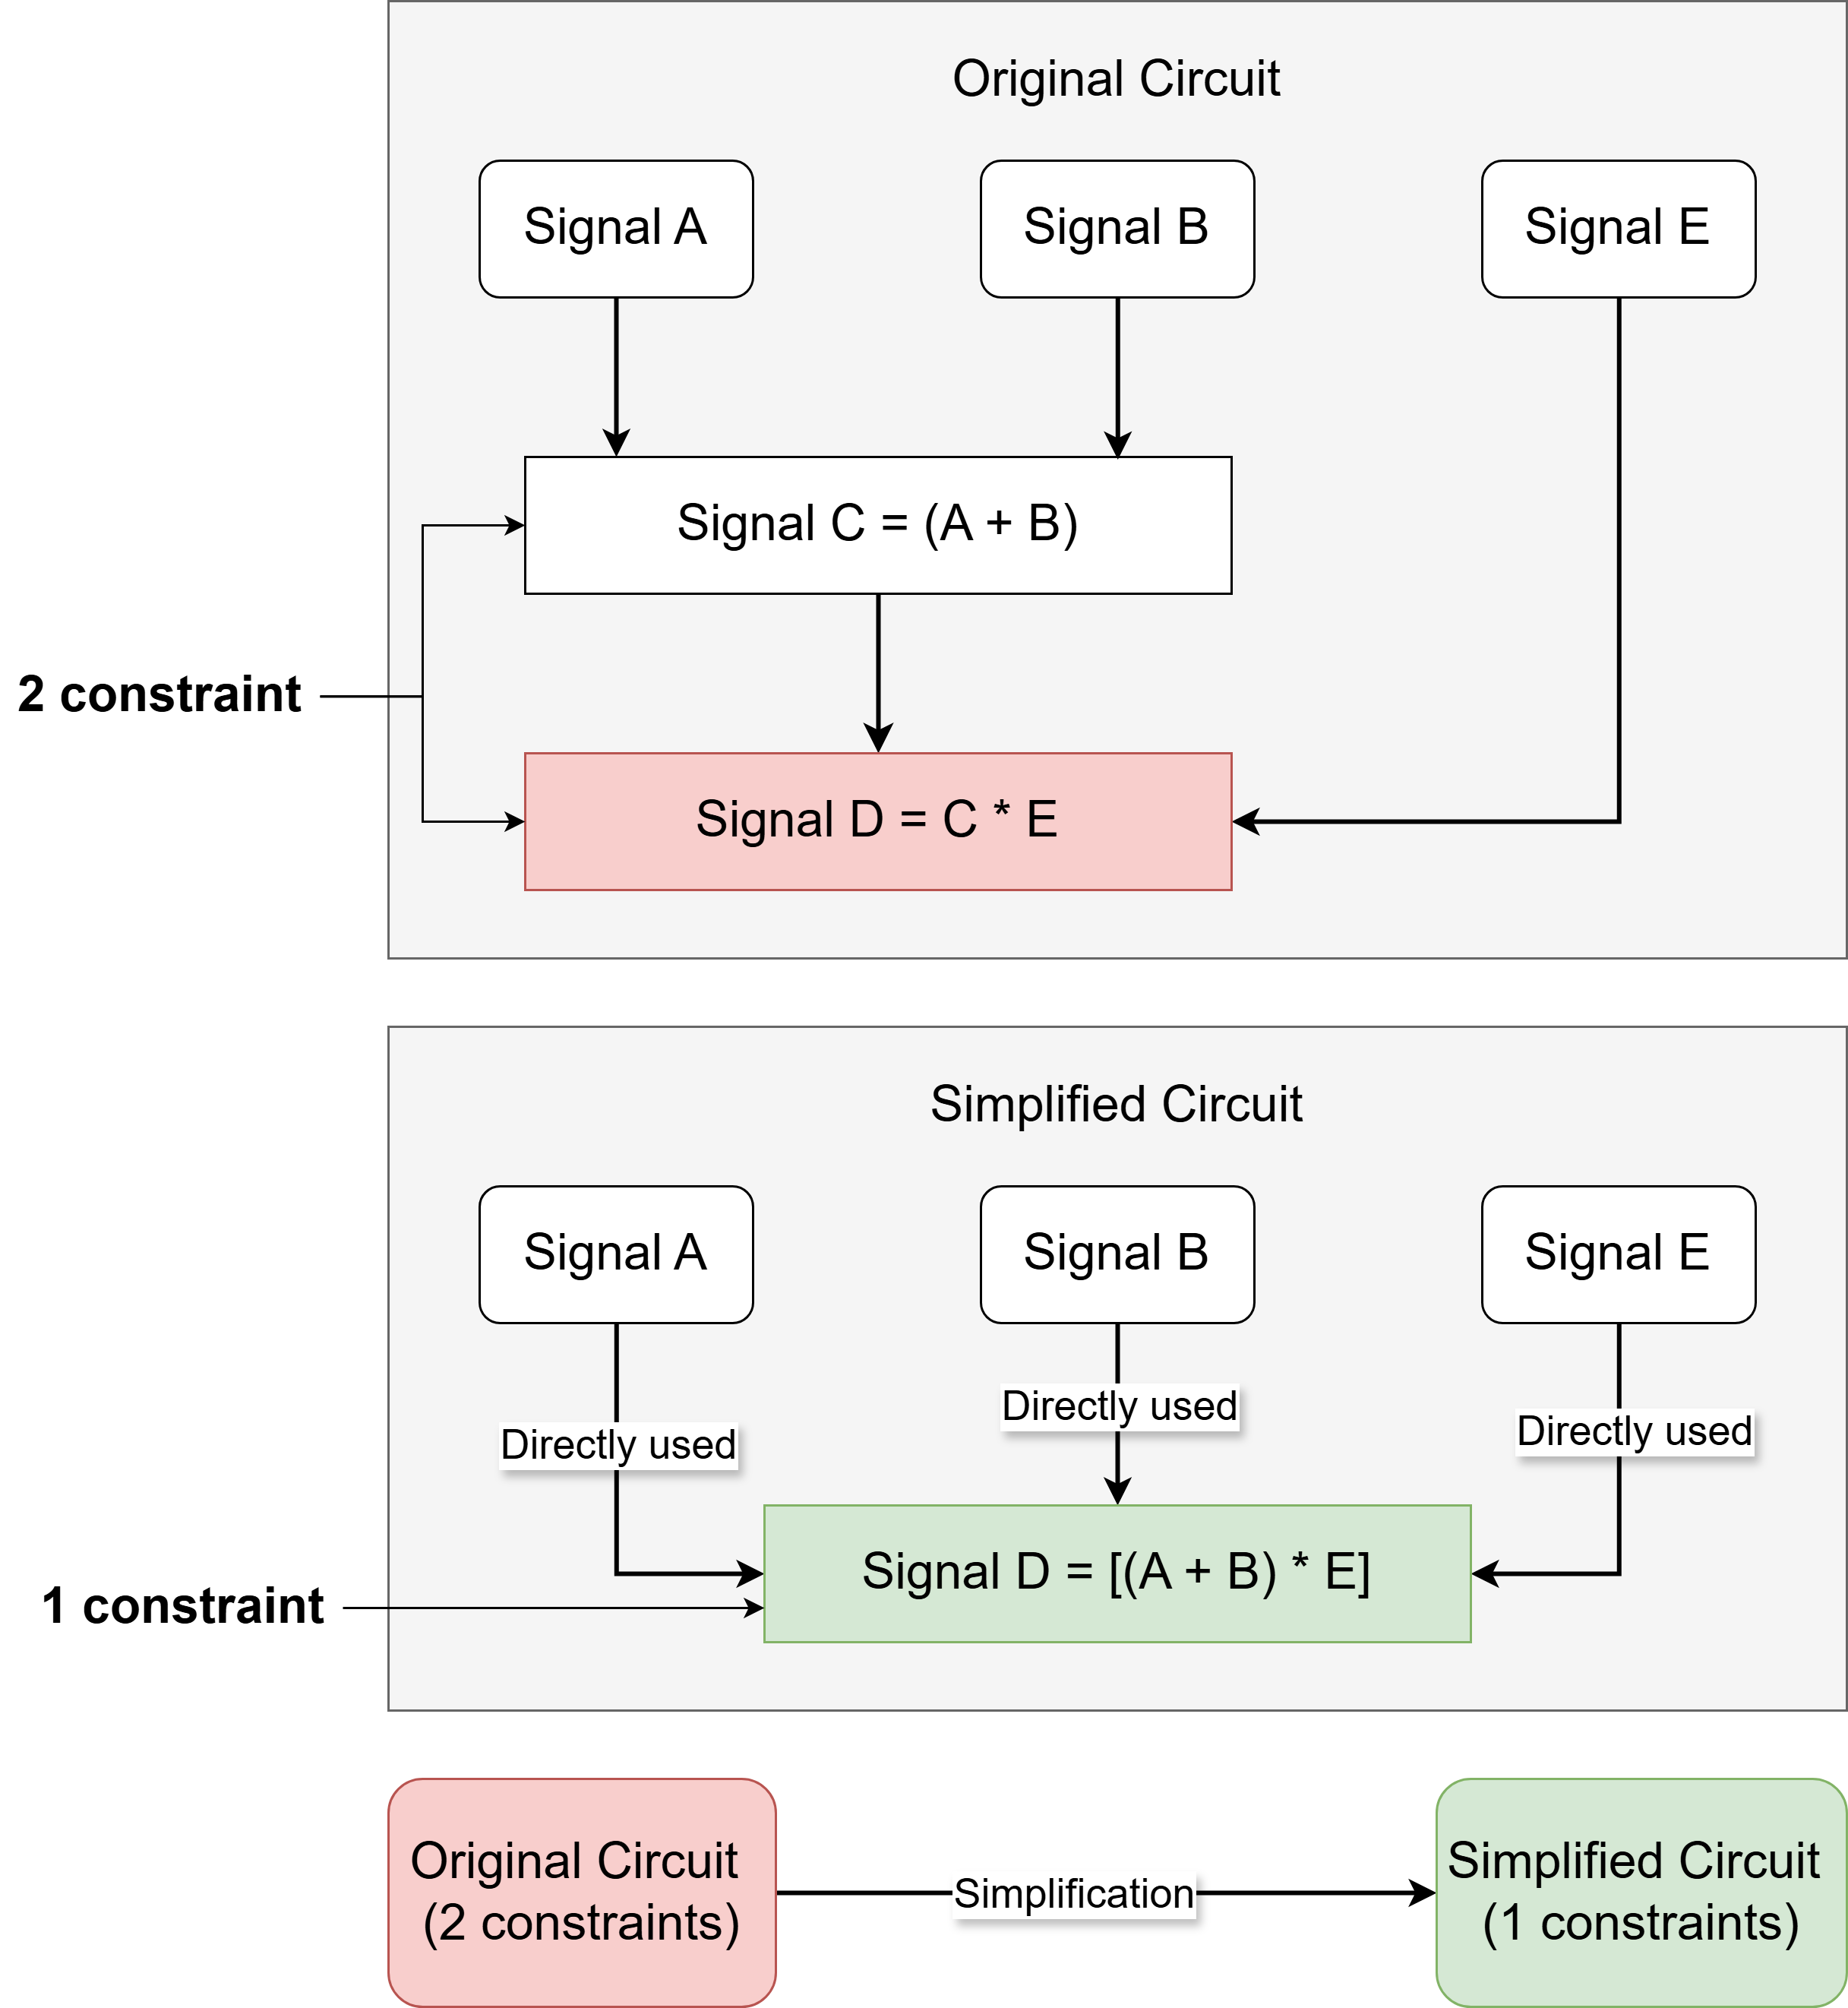
\includegraphics[width = 0.7\textwidth]{imgs/SimplificationExample.png}
    \caption{Lược đồ minh hoạ quá trình tối ưu ràng buộc}
    \label{fig:chapter3-SimplficationExample}
\end{figure}

\section{Phân tích mức tối ưu hóa --O2}

Qua thực nghiệm, nghiên cứu nhận thấy rằng việc sử dụng cờ tối ưu hóa --O2 của trình biên dịch Circom dẫn đến sự gia tăng đáng kể về thời gian biên dịch mạch so với các cờ --O0 và --O1. Đặc biệt hơn, nghiên cứu nhận thấy thời gian thực hiện các vòng lặp khử Gauss không phải là giai đoạn tốn nhiều thời gian nhất trong quá trình tối ưu --O2, mà chính bước khử Gauss đầu tiên trước khi áp dụng các vòng lặp khử Gauss gây tốn nhiều thời gian hơn cả. Để tìm hiểu nguyên nhân, em đã tiến hành phân tích hoạt động của mã nguồn trình biên dịch Circom và nhận thấy rằng sự khác biệt chủ yếu đến từ khối lượng lớn ràng buộc tuyến tính mà bước khử Gauss trong --O2 cần phải xử lí. Dưới đây là phân tích chi tiết:

\subsection{Sự khác biệt cốt lõi trong quy trình tối ưu hóa}

Điểm khác biệt chính giữa --O1 và --O2 nằm ở việc --O2 sử dụng một quy trình tối ưu hóa tuyến tính bổ sung mà --O1 không được áp dụng. 

Với --O1, trình biên dịch chỉ thực hiện các bước đơn giản hóa cơ bản và không áp dụng các thuật toán phức tạp để giảm ràng buộc tuyến tính. Các ràng buộc tuyến tính chỉ được loại bỏ thông qua các phép thay thế đơn giản như đề cập ở \ref{Cơ chế tối ưu hoá ràng buộc trong Circom}. 

Với --O2, trình biên dịch sử dụng một cơ chế đơn giản hóa tuyến tính dựa trên cụm (cluster-based linear simplification). Đây là một hoạt động đòi hỏi nhiều tính toán cùng với lượng lớn ràng buộc tuyến tính cần xử lí là nguyên nhân chính gây ra sự khác biệt về thời gian biên dịch.

\subsection{Các giai đoạn xử lý chung và chi phí}

% Cả --O1 và --O2 đều thực hiện các bước xử lý cơ bản, nhưng chi phí của chúng tăng lên đáng kể khi mạch trở nên phức tạp hơn, đặc biệt là khi các kết quả của các bước xử lý này được sử dụng làm đầu vào cho các bước tối ưu hóa sâu hơn của --O2:

% \begin{itemize}
%     \item \textbf{Xây dựng tập hợp tín hiệu liên quan:} Trình biên dịch cần xác định tất cả các tín hiệu thuộc các ràng buộc phi tuyến và các mối quan hệ phụ thuộc giữa chúng với nhau. Quá trình này bao gồm việc duyệt qua toàn bộ biểu diễn đồ thị của mạch và xác định các tín hiệu cần phải giữ lại.
%     \item \textbf{Khử các ràng buộc đẳng thức đơn giản:} Các ràng buộc đơn giản như \texttt{signal = k} (trong đó \texttt{k} là một hằng số) và \texttt{signal1 = signal2} được xử lý.
%     \item \textbf{Xây dựng lại tập hợp các tín hiệu liên quan:} Tính toán lại các tín hiệu liên quan sau khi áp dụng các phép thế của bước ``Đơn giản hóa các ràng buộc đẳng thức''.
    
% \end{itemize}

Cả hai mức tối ưu –O1 và –O2 đều thực hiện các bước xử lý cơ bản trong quá trình biên dịch, tuy nhiên chi phí xử lý có xu hướng gia tăng đáng kể khi độ phức tạp của mạch tăng lên. Điều này đặc biệt rõ ràng khi các kết quả từ các bước xử lý cơ bản được sử dụng làm đầu vào cho các giai đoạn tối ưu hóa sâu hơn trong –O2.

Bước đầu tiên trình biên dịch thực hiện là xây dựng tập hợp các tín hiệu liên quan. Trình biên dịch cần xác định tất cả các tín hiệu tham gia vào các ràng buộc phi tuyến cũng như các mối quan hệ phụ thuộc giữa chúng. Quá trình này đòi hỏi việc duyệt qua toàn bộ biểu diễn đồ thị của mạch để xác định các tín hiệu cần được giữ lại nhằm đảm bảo tính toàn vẹn trong quá trình đơn giản hóa.

Tiếp theo, trình biên dịch tiến hành khử các ràng buộc đẳng thức đơn giản. Những ràng buộc có dạng như signal = k (với k là một hằng số) hoặc signal1 = signal2 sẽ được xử lý thông qua các phép thay thế trực tiếp, nhằm giảm số lượng ràng buộc một cách hiệu quả mà không ảnh hưởng đến tính đúng đắn của mạch.

Sau khi thực hiện các phép thay thế, trình biên dịch cần xây dựng lại tập hợp các tín hiệu liên quan. Việc này bao gồm việc tính toán lại toàn bộ các tín hiệu còn hoạt động sau khi biểu đồ ràng buộc đã được cập nhật. Quá trình này đảm bảo rằng các bước tối ưu hóa tiếp theo có thể hoạt động trên một tập hợp tín hiệu chính xác và tối thiểu, từ đó nâng cao hiệu quả tối ưu hóa tổng thể.

\subsection{Các hoạt động tối ưu hóa nâng cao của --O2}

Thời gian biên dịch tăng lên đáng kể ở --O2 chủ yếu do các hoạt động tính toán sau đây, được kích hoạt bởi cơ chế tối ưu hóa tuyến tính của --O2:

\begin{itemize}
    \item \textbf{Đơn giản hóa tuyến tính dựa trên cụm:} Đây là hoạt động tối ưu hóa quan trọng nhất của --O2. Trình biên dịch thực hiện khử Gauss với xử lý song song, nhóm các ràng buộc liên quan thành các cụm có chung tín hiệu. Mặc dù việc xử lý song song giúp tăng tốc độ trong các vòng lặp chính, nhưng với khối lượng ràng buộc rất lớn của mạch ZK-Rollup, thời gian xử lí của quá trình này vẫn tăng lên đáng kể.
    \item \textbf{Nhiều vòng lặp tối ưu hóa:} --O2 không chỉ thực hiện tối ưu hóa một lần mà lặp đi lặp lại nhiều vòng cho đến khi không còn ràng buộc tuyến tính nào có thể được đơn giản hóa thêm. Mỗi vòng lặp đòi hỏi việc kiểm tra, xử lý lại các ràng buộc, và đặc biệt là việc xác định khi nào các ràng buộc phi tuyến tính ban đầu trở thành tuyến tính sau các phép thế. Quá trình lặp này làm tăng đáng kể tổng thời gian xử lý.
    \item \textbf{Quản lý cấu trúc dữ liệu:} Để thực hiện các tối ưu hóa sâu, trình biên dịch cần xây dựng và duy trì nhiều cấu trúc dữ liệu trong bộ nhớ để theo dõi các tín hiệu như ràng buộc và các phép thế. Việc quản lý và truy cập liên tục vào các cấu trúc này, đặc biệt với các mạch lớn, tiêu tốn nhiều tài nguyên bộ nhớ và thời gian xử lý.
    \item \textbf{Thay thế và xử lý lại ràng buộc:} Trong mỗi vòng lặp tối ưu hóa, các phép thế được áp dụng cho tất cả các ràng buộc. Sau đó, hệ thống phải kiểm tra lại toàn bộ tập hợp ràng buộc để xác định những ràng buộc nào đã trở thành tuyến tính và cần được xử lý tiếp. Quá trình duyệt và cập nhật liên tục này là một yếu tố chính gây tốn thời gian.
    \item \textbf{Cơ chế kiểm soát vòng lặp:} Mặc dù trình biên dịch có tham số để giới hạn số vòng lặp tối đa, nhưng chính vòng lặp đầu tiên đã chịu phần xử lí nhiều nhất cho lượng lớn ràng buộc tuyến tính làm đầu vào ban đầu.
\end{itemize}

\subsection{Kết luận}

Tóm lại, sự gia tăng đáng kể về thời gian biên dịch của cờ --O2 so với --O0 và --O1 không phải hoàn toàn do các vòng lặp khử Gauss xử lí chậm, mà còn do chi phí thiết lập ban đầu cao trước khi bắt đầu thực hiện các vòng lặp. Các giai đoạn xử lý này bao gồm việc xây dựng các cấu trúc dữ liệu, thực hiện nhiều lần duyệt qua các ràng buộc, và các thao tác bộ nhớ khác trên lượng ràng buộc tuyến tính lớn ở đầu vào. Mặc dù tốn kém về thời gian biên dịch, những chi phí này là cần thiết để đạt được mức độ giảm ràng buộc tối đa, từ đó dẫn đến thời gian tạo bằng chứng nhanh hơn và kích thước bằng chứng nhỏ hơn, điều này đặc biệt quan trọng trong môi trường sản xuất nơi việc tạo bằng chứng được thực hiện thường xuyên.